% PYNE paper series — complete volume (all pages)
% Builds a single PDF that includes every manuscript in order.
% Requires the per-paper main.pdf files (run `make all` from .papers/ first).
%
% Build:  cd .papers/series-complete && tectonic main.tex
%    or:  make series   (from .papers/)
\documentclass[11pt,a4paper]{article}

\usepackage[margin=1in]{geometry}
\usepackage[T1]{fontenc}
\usepackage{times}
\usepackage{xcolor}
\usepackage{hyperref}
\usepackage{bookmark}
\usepackage{pdfpages}
\usepackage{graphicx}
\usepackage{fancyhdr}
\usepackage{tcolorbox}
\usepackage{enumitem}
\usepackage{microtype}

\definecolor{pyneorange}{HTML}{F97316}
\definecolor{pyneblue}{HTML}{2563EB}
\definecolor{pynegray}{HTML}{6B7280}
\definecolor{pynegreen}{HTML}{16A34A}

\hypersetup{
  colorlinks=true,
  linkcolor=pyneblue,
  urlcolor=pyneorange,
  pdftitle={PYNE Academic Paper Series --- Complete Volume},
  pdfauthor={HOOX / PYNE Project},
  pdfsubject={Independent open toolchain for the Pine Script language},
  pdfkeywords={Pine Script, PYNE, compilers, DSL, LSP, technical analysis}
}

\pagestyle{fancy}
\fancyhf{}
\fancyhead[L]{\small\textcolor{pynegray}{PYNE Paper Series}}
\fancyhead[R]{\small\textcolor{pynegray}{Complete Volume}}
\fancyfoot[C]{\thepage}
\renewcommand{\headrulewidth}{0.3pt}

\title{%
  \vspace*{1.5cm}
  {\Large\textcolor{pyneorange}{\textbf{PYNE}}}\\[0.6em]
  {\LARGE\bfseries Academic Paper Series}\\[0.4em]
  {\large Complete Volume --- All Manuscripts}\\[1.2em]
  {\normalsize Independent Open Toolchain for the Pine Script\texttrademark\ Language}
}
\author{%
  HOOX Research / PYNE Contributors\\[0.3em]
  \small Independent Open Source Research\\
  \small \url{https://hoox.sh}
  ~\textperiodcentered~
  \url{https://github.com/hoox-sh/pyne}
}
\date{2026}

\begin{document}

%------------------------------------------------------------------------------
% Front matter
%------------------------------------------------------------------------------
\maketitle
\thispagestyle{empty}

\begin{abstract}
\noindent
This volume concatenates the full set of arXiv-oriented manuscripts describing
\textsc{Pyne} (\texttt{pynescript} / \texttt{hoox-pyne}): architecture, Numba
compilation, series/runtime performance, grammar and ASDL front-end, numerical
parity and strategy semantics, and Language Server Protocol tooling.
Each part is the complete original paper (all pages), included without abridgement.
\end{abstract}

\vspace{0.8em}
\noindent\textbf{Trademark notice.}
Pine Script\texttrademark\ and TradingView\textregistered\ are trademarks of
TradingView, Inc. PYNE is an independent, unofficial implementation and is not
affiliated with, authorized by, sponsored by, or endorsed by TradingView, Inc.

\vspace{1.2em}
\begin{tcolorbox}[
  colback=pyneblue!4,
  colframe=pyneblue!55!black,
  title=\textbf{Volume contents},
  fonttitle=\bfseries,
  boxrule=0.6pt,
  arc=2pt,
  left=4pt,right=4pt,top=2pt,bottom=2pt
]
\begin{enumerate}[leftmargin=1.6em,itemsep=0.45em]
  \item \textbf{Architecture} ---
    \emph{PYNE: An Open Dual-Engine Toolchain for Offline Pine Script Evaluation}
    \hfill {\small\texttt{paper01}}
  \item \textbf{Compiler} ---
    \emph{Compiling Bar-Oriented Trading DSLs to Numba}
    \hfill {\small\texttt{paper02}}
  \item \textbf{Series \& runtime} ---
    \emph{Efficient Series History and Incremental Technical Analysis}
    \hfill {\small\texttt{paper03}}
  \item \textbf{Grammar} ---
    \emph{Formalizing a Charting DSL: ANTLR4 and ASDL for Pine Script}
    \hfill {\small\texttt{paper04}}
  \item \textbf{Parity \& strategy} ---
    \emph{Numerical Parity and Strategy Semantics for Independent Runtimes}
    \hfill {\small\texttt{paper05}}
  \item \textbf{LSP tooling} ---
    \emph{Language Tooling for Financial DSLs: LSP and Multi-Editor Delivery}
    \hfill {\small\texttt{paper06}}
\end{enumerate}
\end{tcolorbox}

\vspace{1em}
\noindent
\textbf{How to rebuild.} From the \texttt{.papers/} directory run
\texttt{make all} (individual papers) then \texttt{make series} (this volume).
Sources live under \texttt{paper01-*}~\ldots~\texttt{paper06-*}; shared macros
and bibliography under \texttt{common/}.

\clearpage
\tableofcontents
\clearpage

%------------------------------------------------------------------------------
% Part I — Architecture
%------------------------------------------------------------------------------
\pdfbookmark[0]{01 Architecture}{part-01}
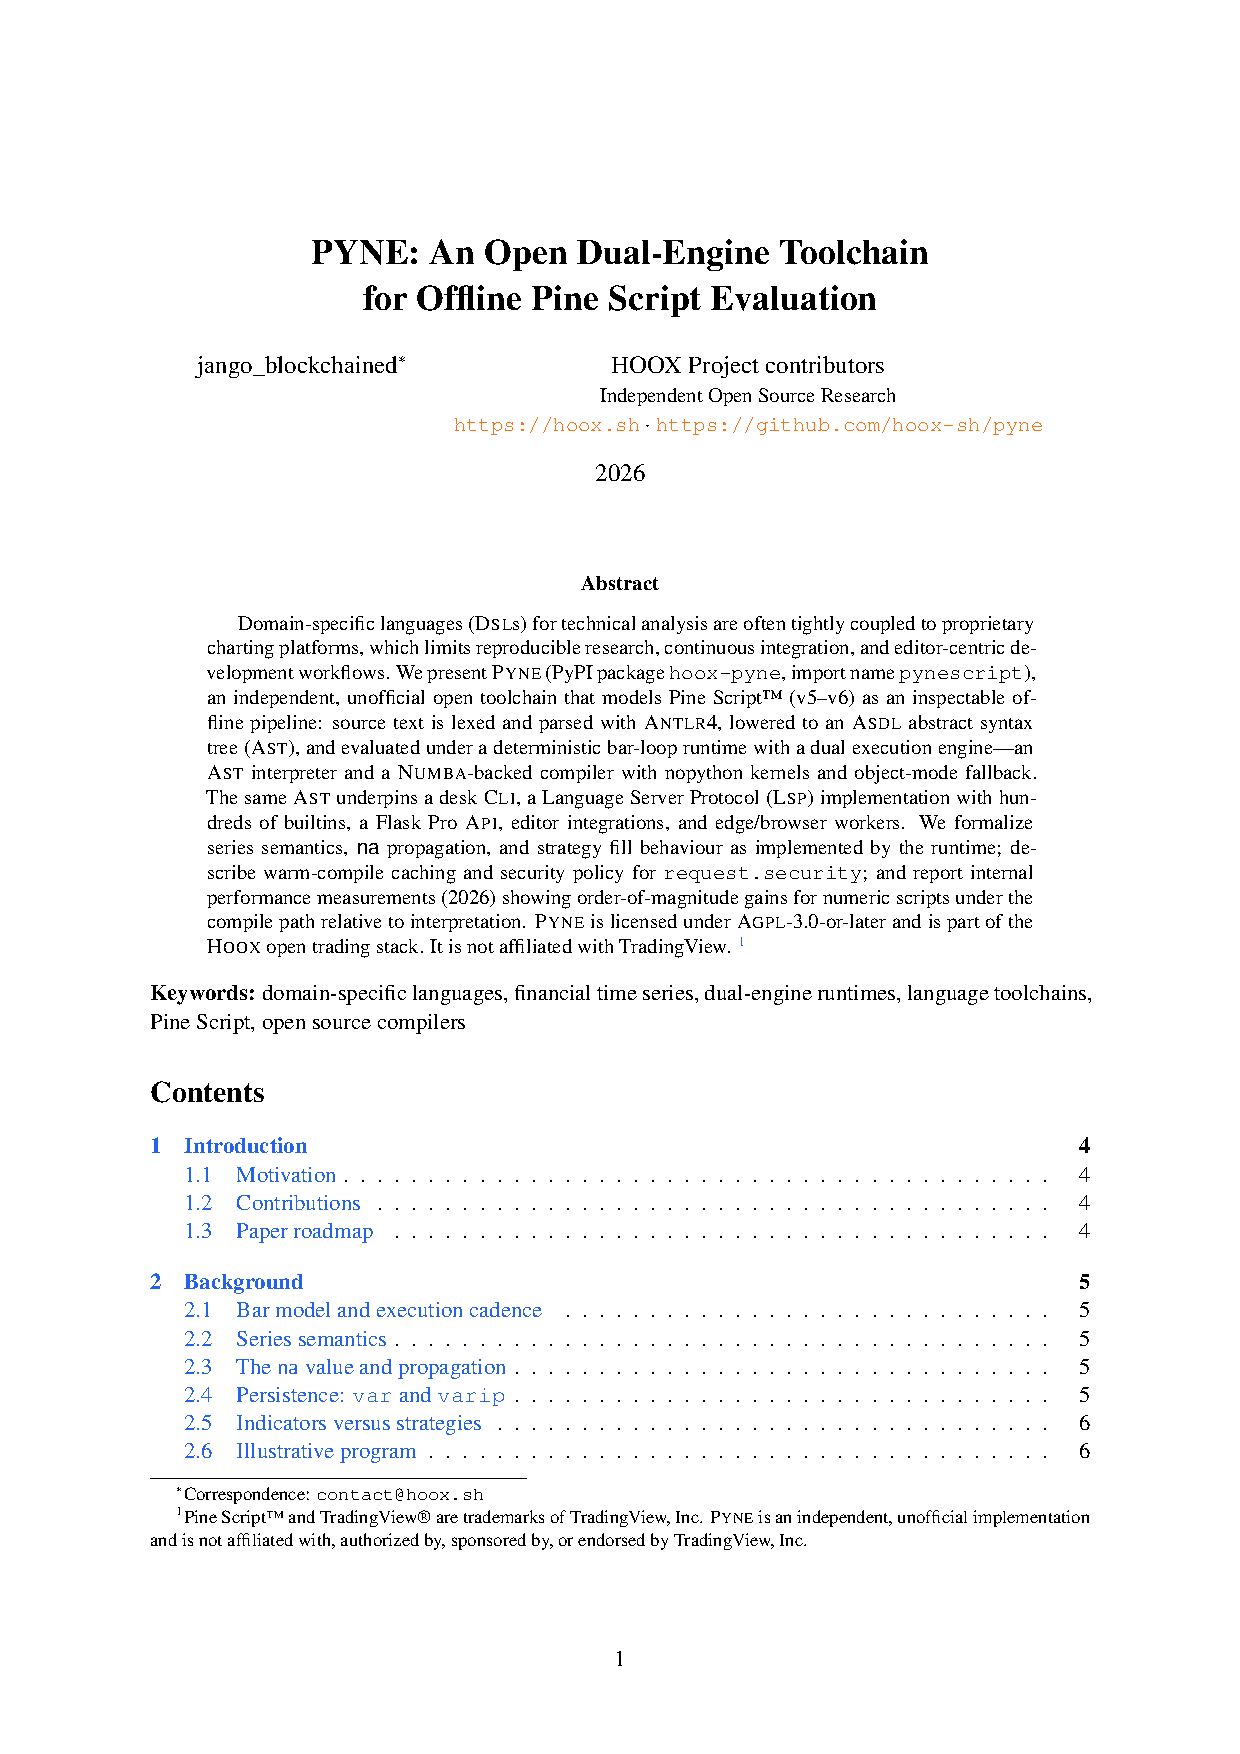
\includepdf[
  pages=-,
  pagecommand={\thispagestyle{fancy}},
  addtotoc={1,section,1,{PYNE: An Open Dual-Engine Toolchain for Offline Pine Script Evaluation},paper01},
  linktodoc=false
]{../paper01-architecture/main.pdf}

%------------------------------------------------------------------------------
% Part II — Compiler
%------------------------------------------------------------------------------
\pdfbookmark[0]{02 Compiler}{part-02}

\includepdf[
  pages=-,
  pagecommand={\thispagestyle{fancy}},
  addtotoc={1,section,1,{Compiling Bar-Oriented Trading DSLs to Numba},paper02},
  linktodoc=false
]{../paper02-compiler/main.pdf}

%------------------------------------------------------------------------------
% Part III — Series \& runtime
%------------------------------------------------------------------------------
\pdfbookmark[0]{03 Series and Runtime}{part-03}

\includepdf[
  pages=-,
  pagecommand={\thispagestyle{fancy}},
  addtotoc={1,section,1,{Efficient Series History and Incremental Technical Analysis},paper03},
  linktodoc=false
]{../paper03-series-runtime/main.pdf}

%------------------------------------------------------------------------------
% Part IV — Grammar
%------------------------------------------------------------------------------
\pdfbookmark[0]{04 Grammar}{part-04}

\includepdf[
  pages=-,
  pagecommand={\thispagestyle{fancy}},
  addtotoc={1,section,1,{Formalizing a Charting DSL: ANTLR4 and ASDL for Pine Script},paper04},
  linktodoc=false
]{../paper04-grammar/main.pdf}

%------------------------------------------------------------------------------
% Part V — Parity \& strategy
%------------------------------------------------------------------------------
\pdfbookmark[0]{05 Parity and Strategy}{part-05}

\includepdf[
  pages=-,
  pagecommand={\thispagestyle{fancy}},
  addtotoc={1,section,1,{Numerical Parity and Strategy Semantics for Independent Runtimes},paper05},
  linktodoc=false
]{../paper05-parity-strategy/main.pdf}

%------------------------------------------------------------------------------
% Part VI — LSP tooling
%------------------------------------------------------------------------------
\pdfbookmark[0]{06 LSP Tooling}{part-06}

\includepdf[
  pages=-,
  pagecommand={\thispagestyle{fancy}},
  addtotoc={1,section,1,{Language Tooling for Financial DSLs: LSP and Multi-Editor Delivery},paper06},
  linktodoc=false
]{../paper06-lsp-tooling/main.pdf}

\end{document}
